
\begin{flushleft}
	
	ASCII (American Standard Code for Information Interchange) is the character encoding format for text data in computers and on the internet.
		
	\begin{figure}[h!]
			\centering
			\includegraphics[scale=.55]{content/chapter2/images/asci.png}
	\end{figure}
	
	English characters are stored using the ascii code and further converted to binary.
	\begin{figure}[h!]
			\centering
			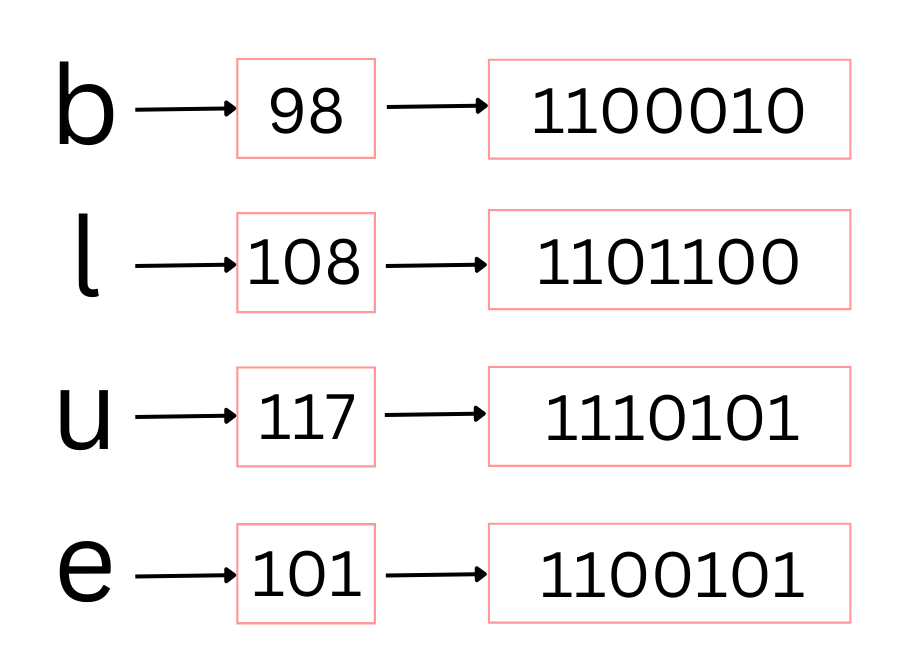
\includegraphics[scale=.12]{content/chapter2/images/ascii.png}
	\end{figure}
	

		
\end{flushleft}

\newpage

